\documentclass[a4paper]{article}
\usepackage[english,spanish]{babel}
\usepackage[utf8]{inputenc}
\usepackage[T1]{fontenc}
\usepackage{verse}
\usepackage[noend]{algpseudocode}
\usepackage{listings}
%% Sets page size and margins
\usepackage[a4paper,top=3cm,bottom=3cm,left=3cm,right=3cm,marginparwidth=1.75cm]{geometry}
%% Useful packages
\usepackage{amsmath}
\usepackage{graphicx}
\usepackage[colorinlistoftodos]{todonotes}
\usepackage[colorlinks=true, allcolors=blue]{hyperref}

\newcommand{\verso}[1] {
\settowidth{\versewidth}{123456789012345678901234567890}%
\begin{minipage}[t]{\dimexpr\versewidth+1pt\relax}
\begin{verse}[\versewidth]
{\fontfamily{qzc}\selectfont\large
  #1
}
\end{verse}
\end{minipage}\bigskip
}

\title{Trabajo Práctico 4}

\begin{document}
\maketitle

\section{Problema A: Armando el polígono}

\subsection{Resolución}

Nuestra tarea es, como bien indica el título: \textit{armar el polígono}.
Nos dan el polígono simple descompuesto en triángulos y la idea es amar el polígono a partir del perímetro que forman estos triángulos.\\
Un polígono es simple cuando sus lados no adyacentes, no se intersecan.
Al ser el conjunto de triángulos que nos dan, una descomposición del polígono original, sabemos que la unión de todos los triángulos es igual al polígono original. También sabemos que los vértices de los triángulos son vértices del polígono original y que para cualquier par de triángulos o bien este par es disjunto o bien comparten un lado o un vértice.\\

Si queremos armar el polígono original, nuestra misión es recorrer está unión de triángulos siguiendo los lados exteriores de los estos triángulos. Es decir, siguiendo aquellos lados que dividen al plano geométrico en dos regiones: la parte interna del polígono y la región exterior a él.\\

\begin{center}
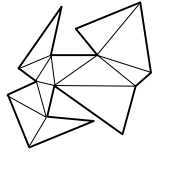
\includegraphics[width=8.5cm,height=6.5cm,keepaspectratio]{poligonoTriangulado.png}
\end{center}

Un primer paso que podemos hacer para dar con la solución al problema es quedarnos con los lados externos de esta triangulación. Como sabemos que para cualquier par de triángulos puede pasar que sean disjuntos o compartan un vértice o compartan un lado. Aquellos lados compartidos, es decir que estén en más de un triangulo, serán lados internos del polígono. Estos lados son los que queremos borrar de la triangulación. A parte sabemos que estos lados internos estarán en exactamente 2 triángulos, pues como mencionamos los triángulos o bien son disjuntos o bien comparten un vértice o un lado entre sí. Si 2 triángulos comparten un lado, ningún otro triángulo puede estar conformado por ese lado. ¿Por qué remarcamos esto? Porque fue parte esencial en nuestro algoritmo para remover lados internos.\\

A continuación detallaremos cómo removimos los lados internos de la triangulación original.
Básicamente leemos del STDIN cada triángulo.
Por cada triángulo, tenemos los 3 puntos pertenecientes al mismo. Con estos armamos los lados del triángulo, que van a ser 3.
En un conjunto vamos agregando cada lado y a la hora de insertar nos fijamos si el lado estaba o no en el conjunto.
Si no estaba, el método $insert$ del set provisto por C++, lo va a agregar al conjunto. Si el lado que queremos agregar ya pertenecía al conjunto, lo borramos del conjunto, pues si es la segunda vez que aparece, es porque ese lado es un lado interno.
Sabemos que esto funciona por lo que mencionamos anteriormente sobre que para todo lado interno, el mismo pertenecerá a 2 triángulos. Caso contrario pertenecerá a un solo triángulo, por lo que ese lado será externo.
Esto lo hacemos en el siguiente código:\\

\begin{lstlisting}[language=c++]
	pair<set<Line>::iterator,bool> inserted;
	inserted = lines.insert(line);
		if(inserted.second==false){
			it = inserted.first;
			lines.erase(it);
		}
\end{lstlisting}

Luego de que tenemos el conjunto de lados de la triangulación sin los lados internos, dar con los puntos del polígono original es una tarea relativamente sencilla.\\

Si tenemos en cuenta la triangulación del polígono de la pagina anterior, luego de remover lados internos la imagen resultante será la siguiente:

\begin{center}
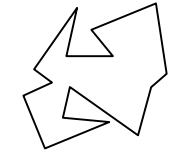
\includegraphics[width=7.5cm,height=5.5cm,keepaspectratio]{poligono.png}
\end{center}

Aunque es evidente, la agregamos para ayudarnos con la explicación del algoritmo.

A continuación queremos dar con los puntos del polígono en orden horario comenzando con el punto que tenga menos coordenada X, y en caso de haber más de uno, desempatar con el de menor coordenada Y.\\

En la siguiente imagen mostramos el punto con menor coordenada X, es decir, el punto más a la izquierda.

\begin{center}
\hspace*{-2cm}
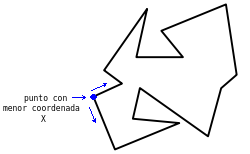
\includegraphics[width=8.5cm,height=7.5cm,keepaspectratio]{poligonoConPuntoMin.png}
\end{center}

Ahora tenemos que ir avanzando por el polígono en sentido horario. Para esto hicimos una función que llamamos $polarOrder$, que nos dice, para un punto de referencia que punto viene primero en orden polar en sentido horario. Esto lo necesitamos para saber para que lado avanzar una vez que tenemos el punto de menor coordenada X. En el gráfico anterior vemos que tenemos dos opciones para elegir.
En nuestro código hacemos lo siguiente:

\begin{lstlisting}[language=c++]
	Point next = min.polarOrder(adj1, adj2) ? adj1 : adj2;
\end{lstlisting}

Parados en el punto de menor coordenada X, llamado $min$, le pasamos a la función polarOrder los puntos  adyacentes al punto $min$. Donde con puntos adyacentes nos referimos a los del otro extremo de los lados que contienen al punto $min$.

Una vez que sabemos que punto es el próximo a $min$, para todos los demás puntos vamos a tener 2 opciones: en un extremo vamos a tener al punto del que venimos y en otro al nuevo punto. Esto nos permite ir avanzando por el polígono simplemente mirando los extremos de cada lado.

Para poder hacer esto, teniendo en cuenta los lados en los que participa cada punto, nos guardamos en un mapa cuales son los puntos que están del otro lado del extremo.

\begin{lstlisting}[language=c++]
	map<Point, set<Point> > adjacents;
	for(it=lines.begin(); it!=lines.end();it++){
		adjacents[it->a].insert(it->b);
		adjacents[it->b].insert(it->a);
	}
\end{lstlisting}

Luego es simplemente avanzar por el polígono hasta volver a encontrarnos con el punto de menor coordenada X. Sabiendo que para todo punto del polígono vamos a tener 2 puntos para elegir, uno va a ser el del que acabamos de venir y el otro el siguiente.\\

\newpage

\subsection{Complejidad}

En la primera parte del algoritmo, leemos los triángulos del STDIN que van a estar dados por 3 puntos.
Con los puntos de los triángulos vamos a formar los lados de los mismo y lo vamos a insertar en un conjunto de lados.
Si el polígono tiene N lados, la cantidad de triángulos internos que tendremos será de N-2 triángulos, esto lo tomamos como un hecho porque lo dice el enunciado. Luego, por cada triángulo, tendremos 3 lados, algunos serán eventualmente repetidos. Pero estaremos haciendo 3*(N-2) $insert$ en el $set$. Cada operación de $insert$ tiene complejidad logarítmica en la cantidad de elementos del conjunto.\\
Por lo tanto como peor caso, la complejidad temporal de realizar las operaciones de inserción en el set será de $O(N log N)$.\\
Cabe aclarara que cuando el lado a insertar se encuentra en el conjunto lo borramos del mismo usando la operación $erase$ pasando el iterador que nos devuelve la función $insert$ lo que nos permite borrar el lado interno en tiempo constante amortizado.\\

Luego de esto buscamos el punto con menor coordenada X (desempatando por el de menor coordenada Y).
Esto lo hacemos en tiempo lineal en la cantidad de elementos del conjunto. Es decir, $O(N)$ donde N es la cantidad de puntos del polígono.\\

Tomando como punto de referencia al punto con menor coordenada X, llamamos a la función $polarOrder$. Esta operación se llama una sola vez, luego para saber para que lado del polígono avanzar (ver figura de la página anterior).
Esta función consta de una serie de operación de comparación y aritmética en tiempo constante.\\

Luego construimos un $map<Point, set<Point> >$ donde $Point$ es un struct que consta de 2 enteros tomando los lados externos del polígono que procesamos anteriormente. Insertamos como clave del mapa a los puntos y como significado el otro extremos del punto. Como nos quedamos con los lados exteriores tendremos como significado los 2 puntos extremos de cada punto del polígono. Esto tiene complejidad temporal $O(N log N)$, pues consta de 2 $\times$ $cantidad de lados$ operaciones de $insert$ y la cantidad de lados externos es igual a la cantidad de puntos del polígono.

Luego usando está estructura y sabiendo para que lado del polígono avanzar, podemos devolver los puntos en tiempo lineal en la cantidad de puntos del polígono. Esto lo hacemos en el siguiente código.

\begin{lstlisting}[language=c++]
	cout << min << endl;
	while(!(next==min)){
		cout << next << endl;
		set<Point> adjacent = adjacents[next];
		set<Point>::iterator itAdj = adjacent.begin();
		Point adj1 = *itAdj;
		++itAdj;
		Point adj2 = *itAdj;
		if(prev==adj1){
			prev = next;
			next = adj2;
		}else{
			prev = next;
			next = adj1;
		}
	}
\end{lstlisting}


La complejidad total del algoritmo es O((N log N) + N + (N log N) + N) = O(N log N), donde N es la cantidad de puntos del polígono.

\newpage
\section{Problema B}
\subsection{Resolución}

Queremos calcular la esperanza $E$ de cuantas veces pasamos por el paso 2 (permutación al azar del arreglo $A[i..N)$, con $0 \leq i < N$  

Para eso, vamos a definir: 
\begin{itemize}
	\item $X_t$: como el número de permutaciones hasta ordenar los últimos t elementos de A, con t = N - i. Es decir $A[i..N)$ 
    \item $Y$: si el elemento mínimo de $A[i..N)$ ($A_{min}$) está en la posición $i$ o no.
\end{itemize} 

Para que $A_{min}$ esté en la primera posición tenemos que seleccionarlo entre todo el resto de los elementos que sean diferentes a él. Entonces tenemos:
\begin{center}
$p(Y) = \frac{Ocurrencias(A_{min})}{t}$ con $t = N - i$.
\end{center}
Por el teorema de la esperanza total, tenemos: $E(X_t) = E(E(X_t|Y))$. Veamos que Y puede tomar sólo dos valores: 1 (si $A_{min}$ está primera posición) ó 0. Entonces podemos calcular la esperanza condicional: \\ 
\begin{center}
$E(X_t|Y=1) = E(X_{t-1}|Y)$ \\
$E(X_t|Y=0) = E(X_{t}) + 1$ 

\end{center}

De esta forma, llegamos a que:  
\begin{equation}
  \text{$E(X_t|Y)$}=\begin{cases}
    \text{$E(X_{t-1}|Y)$}, & \text{con probabilidad $p(Y)$}.\\
    \text{$E(X_t) + 1$}, & \text{con probabilidad $1 - p(Y)$}.
  \end{cases}
\end{equation}

  Ahora, utilizando la esperanza total:
  \begin{center}
  $E(X_t) = E(E(X_t|Y)) = E(X_{t-1}|Y)p(Y) + (E(X_t) + 1)(1-p(Y))$ 
  \end{center}
  y resolvemos despejando $E(X_t)$ llegamos a la siguiente ecuación: 
  \begin{equation}
  E(X_t) = E(X_{t-1}|Y) + \frac{1}{p(Y)} - 1 = E(X_{t-1}|Y) + \frac{t}{Ocurr(A_{min})} - 1
  \end{equation}
  Utilizando esta fórmula vamos a ir resolviendo de forma recursiva calculando la esperanza de los sufijos A[i..N). Esto se puede ver representado en el siguiente fragmento del código
  
\begin{lstlisting}[language=c++]
// Ordenamos el arreglo porque es indiferente el orden para calcular E
// y esto nos va a facilitar calcular las ocurrencias 
 sort(A, A + N); 
 int t, occurs = 0;
 // Caso base de E, siempre usamos al menos una permutacion
 double E = 1.0;
 
 for(int i = size-1; i>=0; i--){
    t = size - i;
    if ((t > 1) && (A[i] == A[i+1])){
        //como A esta ordenado, no me pierdo ninguna ocurrencia
    	occurs++;
    } else {
  	    occurs = 1;
    }
    //Utilizo la formula recursiva de E
    E = E + t/occurs - 1;
 }
\end{lstlisting}
\newpage
\subsection{Complejidad}
Vamos a utilizar la propiedad de que la esperanza no cambia según el ordenamiento del arreglo A, ya que este cambia en cada permutación, para mejorar la complejidad propuesta de $O(N^2)$
\begin{itemize}
\item Ordenamos A en $O(NlogN)$  

\item Recorremos A de atrás para adelante realizando el cálculo de ocurrencias y $E(X_t)$ en $O(n)$
\begin{lstlisting}[language=c++]
   for(int i = size-1; i>=0; i--){
      t = size - i;
      if ((t > 1) && (A[i] == A[i+1])){
          //como A esta ordenado, no me pierdo ninguna ocurrencia
          occurs++;
      } else {
          occurs = 1;
      }
      //Utilizo la formula recursiva de E
      E = E + t/occurs - 1;
   }
\end{lstlisting}
Esto funciona porque al estar en órden, si tenemos elementos repetidos vamos a encontrarlos en posiciones consecutivas. Entonces, no necesitamos recorrer todo el arreglo para calcular las ocurrencias de cada elemento, lo que nos haría tener una complejidad temporal de $O(N^2)$

\end{itemize}
Por lo tanto, tenemos una complejidad total de $O(NlogN)$
                                                        
\newpage
\section{Problema C}

Como vimos en la pista de Leo, sabiendo el punto de abajo de todo a la izquierda, que lo llamo punto de pivot, podemos ir agregando triángulos de 3 vértices buenos, donde uno de ellos es el pivot.
Voy a ir calculando la mejor respuesta (dinámicamente, memorizando y borrando la memorización cada vez que cambio de pivot) que tengo cuando el último triángulo que agrego (yendo en orden antihorario) es el de los puntos de pivot, el punto i, y el j ($i<j$, los recorro también en sentido antihorario). Llamo a este triángulo PIJ.
\\
Entonces, si el triángulo PIJ es el último, el anteúltimo será un triángulo que use también el punto $i$. Luego busco en todos los triángulos anteriores, de la manera PXI, donde $x<i$ será otro punto bueno.
\\
Entonces, lo mejor que puedo hacer para terminar con el triángulo PIJ será poner el mejor triángulo PXI como anteúltimo.
Lo que tengo que ver entonces es puedan ir ambos triángulos, PXI y PIJ, en un polígono convexo. Para eso, debo chequear si el cuadrilátero PXIJ es convexo.
\\
Obviamente también tengo que ver antes que nada que el triángulo PIJ no contenga puntos malos (si no, no puede ir como último, anteúltimo, ni nada). Y que el PXI tampoco tenga puntos malos adentro. Pero esto ya lo calculé previamente. Si el PXI tiene puntos malos la "mejor respuesta" que tiene al triángulo PXI como último es 0.
\\
Ahora, al agregar el triángulo PIJ al PXI, estoy contando a los puntos P e I dos veces. Entonces, debo ver si para el PIJ encuentro otro triángulo como anteúltimo ($mejor$>0) o no. Para eso es esta parte del código:
\begin{lstlisting}[language=c++]
int trian=mejor+cuantosBuenosEnTriangulo(actual[0], actual[i], actual[j])-3;
	if(mejor>0){
		trian++;
	}else{
		trian+=3;
	}
\end{lstlisting}

Luego de ver los mejores polígonos convexos, si encontré alguno la respuesta será al menos 3 (algún triángulo).
Si no, quizás puedo hacer un polígono convexo con 2 puntos adentro. Para chequear esto veo que existan $2$ puntos buenos tales que en no haya un punto malo en el medio de este segmento.
Si existen, la respuesta es $2$, si no, siempre puedo cubir un solo punto (siempre que haya, es decir, siempre y cuando $H>0$).

\newpage
\section{Problema D}

En el problema nos piden que dada una permutaci\'on dada, demos la cantidad de posibles resultados tales que al aplicarle esta permutaci\'on a los equipos las relaciones (partido ganado/perdido) se mantengan.\\
Asi podemos abstraernos y tratar de contar todos los grafos dirigidos tales que para todo par de nodos distintos a y b o bien existe una arista de a a b o bien una en sentido contrario en los cuales al aplicar la permutaci\'on a los nodos, resulta en un grafo isomorfo al original.\\
Llamemos $S(a)$ al resultado de aplicar la permutaci\'on al nodo $a$, y en general $S^i(a)$ al resultado de aplicarla $i$ veces. Tambi\'en diremos que $F(a,b)$ es verdadero si $a$ le gana a $b$.\\
El grafo de la permutaci\'on es un conjunto de ciclos, ya que en todo elemento la cantidad de arista que entran y las que salen son iguales a 1.\\
Si dos equipos se encuentran en un mismo ciclo, y $F(a, b)$ entonces $F(S^i(a), S^i(b))$, luego todas las partidas entre equipos cuya distancia en el ciclo sea la misma tienen que tener el mismo resultado, as\'i que la cantidad de formas de elegir los resultados entre los equipos del mismo ciclo son $2^{c/2}$ siendo $c$ el tama\~no del ciclo (pierde/gana para cada una de estas distancias).\\
Si los dos equipos se encuentran en ciclos distintos de la permutaci\'on (de tama\~nos $c$ y $d$), siendo $a$ un nodo del primero y $b$ uno del segundo, vale que $S^{i+c*x}(a) = S^i(a)$ y $S^{j+d*y}(b) = S^j(b)$. Sabemos que existe un $x$ tal que $c*x \equiv g (d)$ donde $g = gcd(c,d)$, luego $F(S^i(a), S^i(b)) = F(S^{i+d*x}(a), S^{i+d*x}(b)) = F(S^i(a), S^{i+g}(b))$. As\'i que lo \'unico que podemos decidir es $F(a, S^i(b))$ para $a$ y $b$ fijos e $i \in [0, d)$, es decir que tenemos $2^{gcd(c,d)}$ maneras de decidirlo.
Ahora tenemos que calcular esto para para cada uno de los pares de ciclos. Esto nos da un algoritmo que tiene complejidad $O(n^2*log(n))$ ya que podemos tener hasta $n$ ciclos y calcular el $gcd$ es $O(log(n))$. Para conseguir el $O(n*log(n))$ lo que haremos es agrupar los ciclos que tienen igual longitud para evitar hacer tantas cuentas, asi nuestra complejidad pasar\'a a ser $O(x^2log(n))$ donde $x$ es la cantidad de longitudes distintas. Veamos que $x < \sqrt{2n}$. En efecto, si ordenamos la longitudes $l_{1}, l_{2}, ... , l_{x}$, tenemos que:\\
$n = \sum_{i=0}^xl_i \leq \sum_{i=0}^xi = x*(x+1)/2 \rightarrow x^2 < x^2+x = 2n \rightarrow x < \sqrt{2n}$
As\'i el algoritmo tiene complejidad $O(n*log(n)).$



\newpage
\section{Códigos}

\subsection{Problema A}

\begin{lstlisting}[language=c++]
#include<iostream>
#include<set>
#include<map>

using namespace std;

struct Point{
	int x;
	int y;
	Point(int x, int y){
		this->x = x;
		this->y = y;
	}
	Point(){
	}
	bool polarOrder(Point q1, Point q2);
};


inline bool operator<(const Point&a, const Point&b){
		return a.x < b.x || ((a.x==b.x) && (a.y < b.y)); 
}

inline bool operator==(const Point&a, const Point&b){
		return a.x==b.x && a.y==b.y;
}

static int ccw(Point a, Point b, Point c) {
	double area2 = (b.x-a.x)*(c.y-a.y) - (b.y-a.y)*(c.x-a.x);
	if      (area2 < 0) return -1;
	else if (area2 > 0) return +1;
	else                return  0;
}

//orden sentido horario
bool Point::polarOrder(Point q1, Point q2){
	double dx1 = q1.x - x;
	double dy1 = q1.y - y;
	double dx2 = q2.x - x;
	double dy2 = q2.y - y;

	if      (dy1 >= 0 && dy2 < 0) return true;    // q1 above; q2 below
	else if (dy2 >= 0 && dy1 < 0) return false;    // q1 below; q2 above
	else if (dy1 == 0 && dy2 == 0) {            // 3-collinear and horizontal
		if      (dx1 >= 0 && dx2 < 0) return true;
		else if (dx2 >= 0 && dx1 < 0) return false;
		else                          return  false;
	}
	else{
		int ccwRes = ccw(*this, q1, q2);
	    if(ccwRes < 0)
			return true;
		return false;
	}
	return true;
}


struct Line{
	Point a;
	Point b;
	Line(){
	}
	Line(Point c, Point d){
		if(c.x < d.x || ((c.x == d.x) && c.y < d.y)){
			this->a = c;
			this->b = d;
		}else{
			this->a = d;
			this->b = c;
		}
	}
};


inline bool operator<(const Line&c, const Line&d){
		return (c.a < d.a) || (c.a==d.a && c.b < d.b); 
}


int main(){
	
	set<Line> lines;
	int n, nTriangules;
	int x, y;
	cin >> n;
	nTriangules = n - 2;
	set<Line>::iterator it;
	for(int i = 0; i < nTriangules; i++){
			cin >> x >> y;
			Point a = Point(x,y);
			cin >> x >> y;
			Point b = Point(x,y);
			cin >> x >> y;
			Point c = Point(x,y);
			
			Line ab = Line(a,b);
			Line bc = Line(b,c);
			Line ac = Line(a,c);

			pair<set<Line>::iterator,bool> inserted;
			 
			inserted = lines.insert(ab);
			if(inserted.second==false){
				it = inserted.first;
				lines.erase(it);
			}
			
			inserted = lines.insert(bc);
			if(inserted.second==false){
				it = inserted.first;			
				lines.erase(it);
			}
			
			inserted = lines.insert(ac);
			if(inserted.second==false){
				it = inserted.first;
				lines.erase(it);
			}
	}
	
	map<Point, set<Point> > adjacents;
	for(it=lines.begin(); it!=lines.end();it++){
		adjacents[it->a].insert(it->b);
		adjacents[it->b].insert(it->a);
	}
	
	map<Point, set<Point> >::iterator iter = adjacents.begin();
	Point min = iter->first;
	while(iter!=adjacents.end()){
		++iter;
		min = (iter->first < min) ? iter->first : min;
	}
	
	set<Point> adjacent = adjacents.at(min);
	set<Point>::iterator itAdj = adjacent.begin();
	Point adj1 = *itAdj;
	++itAdj;
	Point adj2 = *itAdj;
	
	Point next = min.polarOrder(adj1, adj2) ? adj1 : adj2;
	
	Point prev = min;
	cn(min)
	while(!(next==min)){
		cn(next)
		set<Point> adjacent = adjacents[next];
		set<Point>::iterator itAdj = adjacent.begin();
		Point adj1 = *itAdj;
		++itAdj;
		Point adj2 = *itAdj;
		if(prev==adj1){
			prev = next;
			next = adj2;
		}else{
			prev = next;
			next = adj1;
		}
	}
	cout << endl;
	
	return 0;
}
\end{lstlisting}

\newpage
\subsection{Problema B}

\begin{lstlisting}[language=c++]
#include <iostream>
#include <stdio.h>
#include <cstring>
#include <algorithm>
using namespace std;
#include <iomanip> 

int main()
{
    int N;
    cin >> N;
    // Creo arreglo A
    int A[N];
    memset(A,0,sizeof(A));
    for (int i=0; i<N;i++){
        cin >> A[i];
      }

    // Caso base de E, siempre usamos al menos una permutacion
    double E = 1.0;
    int size = sizeof(A)/sizeof(*A);
    
    // Ordenamos el arreglo porque es indiferente el orden para calcular E
	// y esto nos va a facilitar calcular las ocurrencias 
    sort(A, A + N);

    int occurs = 0;
    int t = 0;
    // Calculo Et basandome en la esparanza Et-1 que me dieron
    // los sub arreglos de tamano t
    for(int i = size-1; i>=0; i--){
    	t = size - i;
    	//como A esta ordenado, no me pierdo ninguna ocurrencia
    	if ((t > 1) && (A[i] == A[i+1])){
    		occurs++;
    	} else {
    		occurs = 1;
    	}
    	E = E+ (double)t/(double)occurs - 1;
    }
    
    // Le sumo 1 a la E porque siempre se usa una vez
    cout << setprecision(6) << fixed << E << endl;

    return 0;
}


\end{lstlisting}

\newpage
\subsection{Problema C}

\begin{lstlisting}[language=c++]

#include<iostream>
#include<math.h>
#include<algorithm>
#include<string>
#include<map>
#include<vector>
#include<queue>
#include<stack>

using namespace std;

#define forn(i,n) for(int i=0;i<(int)(n); i++)
#define forsn(i,s,n) for(int i=(s);i<(int)(n); i++)
#define pb push_back
#define mp make_pair

typedef long long tint;

struct point{
	tint x, y;
	
	bool operator <(const point &p) const {
		return y < p.y || (y == p.y && x < p.x);
	}
	
	point(tint x, tint y){
		this->x=x;
		this->y=y;
	}
};

tint cross(point a, point b){
	return (a.x*b.y)-(a.y*b.x);
}

vector<point> h, e;

tint sign (point p1, point p2, point p3)
{
    return (p1.x - p3.x) * (p2.y - p3.y) - (p2.x - p3.x) * (p1.y - p3.y);
}

bool pointInTriangle (point pt, point v1, point v2, point v3)
{
    bool b1, b2, b3;

    b1 = sign(pt, v1, v2) < 0;
    b2 = sign(pt, v2, v3) < 0;
    b3 = sign(pt, v3, v1) < 0;

    return ((b1 == b2) && (b2 == b3));
}

int cuantosBuenosEnTriangulo(point a, point b, point c){
	int cant=0;
	forn(i, h.size()){
		if(pointInTriangle(h[i], a, b, c)){
			cant++;
		}
	}
	return cant;
}

bool hayMalos(point a, point b, point c){
	forn(i, e.size()){
		if(pointInTriangle(e[i], a, b, c)){
			return true;
		}
	}
	return false;
}

bool esConvex(point a, point b, point c, point d){
	vector<point> v; v.pb(a); v.pb(b); v.pb(c); v.pb(d);
	int sig;
	
	 
	forn(i, 4){
		int dx1 = v[(i+1)%4].x-v[(i)%4].x;
		int dy1 = v[(i+1)%4].y-v[(i)%4].y;
		int dx2 = v[(i+2)%4].x-v[(i+1)%4].x;
		int dy2 = v[(i+2)%4].y-v[(i+1)%4].y;
		int zcrossproduct = dx1*dy2 - dy1*dx2;
		//int s = cross(v[i], v[(i+1)%4]);
		//s=(s>=0);
		int s=(zcrossproduct>=0);
		if(i==0){
			sig=s;
		}else{
			if(sig!=s){
				return false;
			}
		}
	}
	return true;
}

vector< vector<int> > dp;
vector< vector<bool> > pase;

int findMejorConUltimo(vector< point > actual, int i, int j){
	if (pase[i][j]){
		return dp[i][j];
	}
	int mejor = 0;
	forsn(a, 1, i){
		if (esConvex(actual[0], actual[a], actual[i], actual[j]) && !hayMalos(actual[0], actual[a], actual[i])){
			mejor=max(mejor, findMejorConUltimo(actual, a, i));
		}
	}
	int trian=mejor+cuantosBuenosEnTriangulo(actual[0], actual[i], actual[j])-3;
	if(mejor>0){
		trian++;
	}else{
		trian+=3;
	}
	dp[i][j]=trian;
	pase[i][j]=true;
	return dp[i][j];
}

int findMax(vector< point > actual){
	forsn(i, 1, actual.size()){
		vector<int> v(actual.size(), 0);
		dp.pb(v);
		vector<bool> v2(actual.size(), false);
		pase.pb(v2);
	}
	int ans=0;
	forsn(i, 1, actual.size()){
		forsn(j, i+1, actual.size()){
			if(!hayMalos(actual[0], actual[i], actual[j])){
				ans=max(ans, findMejorConUltimo(actual, i, j));
			}
		}
	}
	return ans;
}

point pivot(0, 0);

bool orden(point a, point b){
	a.y-=pivot.y;
	a.x-=pivot.x;
	b.y-=pivot.y;
	b.x-=pivot.x;
    if(a.y == 0 and a.x > 0) return true; //angle of p1 is 0, thus p2>p1
    if(b.y == 0 and b.x > 0) return false; //angle of p2 is 0 , thus p1>p2
    if(a.y > 0 and b.y < 0) return true; //p1 is between 0 and 180, p2 between 180 and 360
    if(a.y < 0 and b.y > 0) return false;
    return (cross(a, b))>0; //return true if p1 is clockwise from p2
}

int checkWith(int p){
	vector< point > actual;
	pivot=h[p];
	forn(i, h.size()){
		if(i==p)continue;
		if (h[i].y>h[p].y || (h[i].y==h[p].y && h[i].x>=h[p].x)){
			actual.pb(h[i]);
			//actual.pb(mp(mp(ang, dist), h[i]));
		}
	}
	sort(actual.begin(), actual.end(), orden);
	vector< point > puntos;
	puntos.pb(h[p]);
	forn(i, actual.size()){
		puntos.pb(actual[i]);
	}
	if(puntos.size()<3)return 0;
	return findMax(puntos);
}

bool areCollinear(point a, point b, point c){
	return (a.x*(b.y-c.y) + b.x*(c.y-a.y) + c.x*(a.y-b.y))==0;
}


int main (){
	int H, E;
	cin>>H>>E;
	forn(i, H+E){
		tint a, b;
		cin>>a>>b;
		point pp=point(a, b);
		if(i<H){
			h.pb(point(a, b));
		} else {
			e.pb(point(a, b));
		}
	}
	int ans=0;
	forn(i, H){
		dp.clear();
		pase.clear();
		ans=max(ans, checkWith(i));
	}
	if(ans>0){
		cout<<ans<<endl;
	}else{
		forn(i, H){
			forsn(j, i+1, H){
				bool puedo=true;
				forn(malo, E){
					if(areCollinear(h[i], h[j], e[malo]) && ((h[i].y<e[malo].y && h[j].y>e[malo].y) || (h[i].x<e[malo].x && h[j].x>e[malo].x))){
						puedo=false;
					}
				}
				if(puedo){
					cout<<2<<endl;
					return 0;
				}
			}
		}
		if(H>0){
			cout<<1<<endl;
		}else{
			cout<<0<<endl;
		}
	}
}


\end{lstlisting}

\newpage
\subsection{Problema D}

\begin{lstlisting}[language=c++]
#include <bits/stdc++.h>

using namespace std;

typedef long long int ll;

int n;
vector<int> perm;
const long long int MOD = 1000000007;

void loadValues(){
    cin >> n;
    perm = vector<int>(n);
    
    for(int i=0; i<n; i++){
        cin >> perm[i];
        perm[i]--;
    }
}

ll gcd(ll x, ll y){
    if (y == 0)
        return x;
    else
        return gcd(y, x%y);
}

ll modpow(ll base, ll e){
    if(e == 0) return 1LL;
    ll res = modpow(base, e/2);
    res = (res * res) % MOD;
    if(e%2 == 1) res = (res * base) % MOD;
    return res;
}

// Devuelve los ciclos que contiene el grafo de la permutacion
// Los devuelve ordenados por el largo. Complejidad O(n*log(n))
vector<int> getLoops(){
    vector<int> res;
    vector<bool> visited(n);
    for(int i=0; i<n; i++){
        if(!visited[i]){
            int j = i;
            int size = 0;
            while(!visited[j]){
                visited[j] = true;
                size++;
                j = perm[j];
            }
            res.push_back(size);
        }
    }
    sort(begin(res), end(res));
    return res;
}

// Para cada largo de ciclo, cuenta la cantidad. Complejidad O(n)
vector<pair<int, int>> getSizeXCount(vector<int>& loops){
    vector<pair<int, int>> res;
    
    int count = 0;
    for(int i = 0; i < (int)loops.size(); i++){
        count++;
        if (i == (int)loops.size()-1 || loops[i] != loops[i+1]){
            res.emplace_back(loops[i], count);
            count = 0;
        }
    }
    return res;
}

ll compute(vector<pair<int, int>> sizeXCount){
    ll res = 1LL;
    for(int i = 0; i < (int) sizeXCount.size(); i++){
        int size1 = sizeXCount[i].first;
        ll cant1 = (ll) sizeXCount[i].second;
        
        res *= modpow(modpow(2, size1), cant1*(cant1-1)/2);
        res %= MOD;
        res *= modpow(modpow(2, size1/2), cant1);
        res %= MOD;

        for(int j = i+1; j < (int)sizeXCount.size(); j++){
            int size2 = sizeXCount[j].first;
            ll cant2 = (ll) sizeXCount[j].second;
            
            res *= modpow(modpow(2, gcd(size1, size2)), cant1*cant2);
            res %= MOD;
        }
    }
    return res;
}

int main(){
    
    loadValues();
    vector<int> loops = getLoops();
    vector<pair<int, int>> sizeXCount = getSizeXCount(loops);
    cout << compute(sizeXCount) << endl;
}

\end{lstlisting}

\end{document}